%
% Article for documents at The Hague University
% of Applied Sciences, Electrical Engineering.
%
% (c)2013-2018, J. op den Brouw <J.E.J.opdenBrouw@hhs.nl>
% v0.5b
%
% Versies 0.1 - 0.3 zijn verschenen als Word-documenten
%
% version 0.4a - changed bib from bibtex to biber
%                changed source code formatting using lstlisting
%                minor spelling corrections
%         0.5  - major changes. changed url link to bibtex info
%         0.5a - minor changes and typos
%         0.5b - adjusted spacing (also with some chapternames), because
%                of changed parskip, typos

%% 12pt charachters, A4 paper size, one side printing, equation left aligned
%% equation indent at 0 em
\documentclass[12pt,a4paper,final,twoside,fleqn]{article}
%% Set input encoding to UTF-8
\usepackage[utf8]{inputenc}
%% Use T1 output font encoding
\usepackage[T1]{fontenc}

%% Credentials
\author{Jesse op den Brouw}
\title{C coderen op de AVR ATmega}
\newcommand{\subtitle}{Een aantal praktische tips en voorbeelden voor goede codeertechnieken op de AVR ATmega microcontroller.}
\date{\today}
\newcommand{\version}{0.5b}
%% My email address, nicely in a href
\newcommand\emailaddress{\href{mailto:J.E.J.opdenBrouw@hhs.nl}{\sffamily J.E.J.opdenBrouw@hhs.nl}}


%% PDF Version and compression...
\pdfminorversion=5
\pdfobjcompresslevel=2

%% Dutch spelling of chapter, section, etc.
% http://archive.cs.uu.nl/mirror/CTAN/macros/latex/contrib/csquotes/csquotes.pdf
% standaard Nederlandse quotes zijn old-fashioned (openen laag)
\usepackage[dutch]{babel}
\usepackage[style=english]{csquotes}

%% Set page layout
\usepackage[a4paper,bindingoffset=0.2in,left=1in,right=1in,top=1in,bottom=1.4in,footskip=0.6in]{geometry}

%% Parskip et al.
\usepackage{parskip}[=v1]

%% Allows increasing the font size of specific fonts beyond LaTeX default specifications
\usepackage{anyfontsize}

%% Use appendix
%%\usepackage{appendix}

%% Use of dashed lines in tables
%\usepackage{arydshln}

%% Create text-wrapped figures and tables
\usepackage{wrapfig}

%% Include graphics files
\usepackage{graphicx}

%% Enumerate items
\usepackage{enumitem}

%% Use the AMS Mathematical characters
\usepackage{mathtools}
\usepackage{amsfonts}
\usepackage{amssymb}
\setlength{\mathindent}{1em}

%% Define and use colors
\usepackage{xcolor}

%% Use the Helvetica (~ Arial) font
%\usepackage{helvet}

%% Use the Latin Modern font... Does this change the Math font?
%%\usepackage{lmodern}
%\usepackage{charter}
\usepackage[bitstream-charter]{mathdesign}


%% Default monospaced font from Palatino, e.g. listings
%\renewcommand{\ttdefault}{pcr}
%% Use computer code listings
\usepackage{listings}
\usepackage[scaled=0.85]{beramono}


%% Change the way chapters and sections are formatted, only sections and subsections are used
%%%\usepackage{titlesec}
%%%\titleformat{\section}{\fontfamily{phv}\selectfont\large\bfseries\slshape}{\thesection.}{0.5em}{}
%%%\titleformat{\subsection}{\fontfamily{phv}\selectfont\bfseries}{\thesubsection}{0.5em}{}
%% Change the way chapters and sections are formatted.
\usepackage{titlesec}
\titleformat{\chapter}[hang] 
{\fontfamily{phv}\selectfont\Huge\bfseries\scshape}{\thechapter.}{0.5em}{}
\titleformat{\section}{\fontfamily{phv}\selectfont\large\bfseries}{\thesection}{1em}{}
\titleformat{\subsection}{\fontfamily{phv}\selectfont\bfseries}{\thesubsection}{1em}{}
\titlespacing*{\chapter}{0pt}{25pt}{15pt}
%\titlespacing*{\section}{0pt}{17pt}{3pt}
\titlespacing*{\section}{0pt}{1.0\baselineskip}{0.0\baselineskip}
%\titlespacing*{\subsection}{0pt}{12pt}{1pt}
\titlespacing*{\subsection}{0pt}{\baselineskip}{0.851\baselineskip}
\titlespacing*{\subsubsection}{0pt}{\parskip}{-\parskip}

%% Fancy headers and footers...
\setlength{\headheight}{14.5pt}
\usepackage{fancyhdr}
\pagestyle{fancy}
%%%\lhead{}
%%%\chead{}
%%%\rhead{CONCEPT}
%%%\lfoot{Coderen op de AVR}
%%%\cfoot{}
%%%\rfoot{\thepage}
%%%\renewcommand{\headrulewidth}{0pt}
%%%\renewcommand{\footrulewidth}{0.4pt}
%%%\fancyhead{} % clear all header fields
\fancyhead{}
\fancyhead[LE,RO]{CONCEPT}
\fancyfoot{} % clear all footer fields
\fancyfoot[LE,RO]{\thepage}           % page number in "outer" position of footer line
\fancyfoot[RE,LO]{C coderen op de AVR ATmega} % other info in "inner" position of footer line
\renewcommand{\headrulewidth}{0pt} % no line in header area
\renewcommand{\footrulewidth}{0.4pt} % 0.4pt line


%\renewcommand{\footnoterule}{%
%  \kern -3pt
%  \hrule width \textwidth height 1pt
%  \kern 2pt
%}

%% Indexing words...
\usepackage{imakeidx}
\makeindex

%% Making captions nicer...
\usepackage[font=footnotesize,format=plain,labelfont=bf,up,textfont=sl,up]{caption}

%% For using footnotes in section headers...
% http://archive.cs.uu.nl/mirror/CTAN/macros/latex/contrib/footmisc/footmisc.pdf
% ruimte onder aan de pagina tussen tekst en voetnoot niet na voetnoot
\usepackage[bottom,hang,multiple]{footmisc}
% inspringen
\setlength{\footnotemargin}{1em}
% ruimte tussen footnotes:
\setlength{\footnotesep}{0.7\baselineskip}
% http://archive.cs.uu.nl/mirror/CTAN/macros/latex/contrib/biblatex/doc/biblatex.pdf
%%%%\usepackage[%
%%%%    backend=biber,%
%%%%    backref=true,%
%%%%    style=numeric,sortcites%
%%%%]{biblatex}
%%%%\addbibresource{CoderenopAVR.bib}
\usepackage[
    backend=biber,
    backref=true,
    backrefstyle=none, % neem paginanummer niet samen in de backref lijst dus 1,2,3 i.p.v. 1-3 (anders kun je niet op 2 klikken)
    sortcites=true,
    sorting=none,
    doi = false % doi informatie wordt niet weergegeven
]{biblatex}
\addbibresource{CoderenopAVR.bib}
\DefineBibliographyStrings{dutch}{
    backrefpage = {blz.},
    backrefpages = {blz.},
}

%% Using hyperrefs...
\usepackage{hyperref}
\hypersetup{
	colorlinks=true,
	linkcolor=blue,
    pdftitle={C coderen op de AVR ATmega},    % title
    pdfauthor={J.E.J op den Brouw},     % author
    pdfsubject={Een aantal praktische tips en voorbeelden voor goede codeertechnieken op de AVR microcontroller.},   % subject of the document
    %pdfcreator={Latex},   % creator of the document
    %pdfproducer={PDFtoLaTex}, % producer of the document
    pdfkeywords={AVR}{C coding}{tips and tricks}, % list of keywords
    pdfdisplaydoctitle=true,
	pdfpagelayout=TwoPageRight
}
\renewcommand\UrlFont{\fontfamily{phv}\selectfont}

%%% No package loading from here

%% Create our own maketitle macro
\makeatletter
\def\maketitle{%
  \null
  \thispagestyle{empty}%
  \vfill
  \begin{center}\leavevmode
    {\fontfamily{phv}\fontsize{30pt}{36pt}\selectfont\bfseries\scshape \@title\par}%
    \vskip 1.0cm
    {\fontfamily{phv}\fontsize{13pt}{16pt}\selectfont\bfseries\scshape \subtitle\par}%
    \vskip 8.0cm
    \begin{minipage}[c]{.50\linewidth}
       
\includegraphics[width=\linewidth]{HHS_grijs_groen_fc}
    \end{minipage}\hfill
    \begin{minipage}[c]{0.40\linewidth}
       {\hfill \large \@author\par}%
       \vskip 0.03cm
       {\hfill \large De Haagse Hogeschool\par}%
       \vskip 0.03cm
       {\hfill \large \@date\par}%
       \vskip 0.03cm
       {\hfill \large Versie \version\par}%
       \vskip 0.03cm
       {\hfill \large \emailaddress\par}%
  \end{minipage}
  \end{center}%
  \vfill
  \null
  %%\cleardoublepage
  }
\makeatother

%% Define some colors
\definecolor{dkgreen}{rgb}{0,0.6,0}
\definecolor{gray}{rgb}{0.5,0.5,0.5}
\definecolor{mauve}{rgb}{0.58,0,0.82}
\definecolor{lightgray}{rgb}{0.95,0.95,0.95}
\definecolor{avrstudioioregisters}{RGB}{160,18,87}
\definecolor{avrstudiocomment}{RGB}{4,128,55}
\definecolor{avrstudiostring}{RGB}{128,0,0}
\definecolor{avrstudiospecials}{RGB}{0,0,128}


\definecolor{green}{RGB}{0,128,0}
\definecolor{darkred}{RGB}{163,21,21}
% http://archive.cs.uu.nl/mirror/CTAN/macros/latex/contrib/listings/listings.pdf
\usepackage{listings}
\lstdefinelanguage[AVR]{Assembler}{
morekeywords=[1]{adc,add,adiw,andi,asr,bclr,bld,brbc,brbs,brcc,brcs,break,breq,brge,brhc,brhs,brid,brie,brlo,brlt,brmi,brne,brpl,brsh,brtc,brts,brvc,brvs,bset,bst,cbi,cbr,clc,clh,cli,cln,clr,cls,clt,clv,clz,com,count,cp,cpc,cpi,cpse,dec,eicall,eijmp,elpm,end,eor,espm,fmul,fmuls,fmulsu,in,inc,jmp,ld,ldd,ldi,lds,lsl,lsr,mov,movw,neg,nop,ori,out,pop,push,rcall,ret,reti,rjmp,rol,sbc,sbci,sbi,sbic,sbis,sbiw,sbr,sbrc,sbrs,sec,seh,sei,sen,ser,ses,sev,sez,sleep,st,std,sts,sub,subi,swap,tst,wdr},
morekeywords=[2]{.byte,.cseg,.csegsize,.db,.device,.dseg,.dw,.endm,.equ,.eseg,.exit,.include,.includepath,.listmac,.macro,.nolist,.org,.set,.define,.undef,.ifdef,.ifndef,.else,.elseif,.elif,.message,.warning,.error,byte1,byte2,byte3,byte4,exp2,high,hwrd,log2,low,lwrd,page},
alsoletter=.,
sensitive=false,
morecomment=[l]{\#},
morecomment=[l]{;},
morestring=[b]{"},
morestring=[b]{'}
}[keywords,comments,strings]

\lstset{
    %inputencoding={utf8}, %werkt niet
    %TODO: uitbreiden
    literate={ë}{{\"e}}1 {ï}{{\"i}}1 {é}{{\'e}}1,
    basicstyle=\ttfamily\small,
    tabsize=4,
    identifierstyle=,
    showstringspaces=false,
    commentstyle=\color{green},
    numbers=left,
    numberstyle=\tiny\color{gray},
    breaklines=true,
    captionpos=b,
    abovecaptionskip=.6\baselineskip,
    % niet teveel ruimte onder listing na caption
    % nu exact gelijk aan ruimte onder caption van figure (float)
    belowcaptionskip=.1\baselineskip,
    backgroundcolor=\color{lightgray},
    frame=lines,
    escapeinside={(*@}{@*)},              % escape to Latex using (*@ ...  @*)
    aboveskip=0pt,
    belowskip=0pt
}
% In dit document worden twee programmeertalen gebruikt.
\lstdefinestyle{AVR}{
    language=[AVR]Assembler,
    stringstyle=\color{black},
    keywordstyle=[1]\color{blue},
    keywordstyle=[2]\color{black},
}
\lstdefinestyle{C}{
    language=C,
    stringstyle=\color{avrstudiostring},
    keywordstyle=\color{blue},
    morekeywords={uint8_t,int8_t,uint16_t,int16_t,uint32_t,int32_t,uint64_t,int64_t,asm},
    keywords=[2]{TCCR3A,TCCR3B,TCNT3H,TCNT3L,OCR3AH,OCR3AL,OCR3BH,OCR3BL,ICR3H,ICR3L,ETIMSK,ETIFR,PCMSK1,
    PCMSK0,CLKPR,SREG,SPH,SPL,UCSR1C,UBRR1H,
    EIMSK,GIMSK,GICR,GIFR,TIMSK,TIFR,SPMCR,EMCUCR,MCUCSR,TCCR0,TCNT0,OCR0,SFIOR,TCCR1A,TCCR1B,TCNT1,TCNT1H,
    TCNT1L,OCR1A,OCR1AH,OCR1AL,OCR1B,OCR1BH,OCR1BL,TCCR2,ASSR,ICR1H,ICR1L,TCNT2,OCR2,WDTCR,UBRRHI,UCSROC,UBRROH,
    UBRRH,UBRRL,UCSRA,UCSRB,UCSRC,ADCSRA,ADC,ADCH,ADCL,ADMUX,
    EEAR,EEARH,EEARL,EEDR,EECR,PORTA,DDRA,PINA,PORTB,DDRB,PINB,PORTC,DDRC,PINC,PORTD,DDRD,PIND,SPDR,SPSR,
    SPCR,UDR0,UDR,UCSR0A,USRUCSR0B,UCR,UBRR0,UBRR0L,UBRR,ACSR,PORTE,DDRE,PINE,OSCCAL,UDR1,UCSR1A,
    UCSR1B,UBRR1,UBRR1L,COM3A1,COM3A0,COM3B1,COM3B0,FOC3A,FOC3B,WGM31,WGM30,ICNC3,ICES3,WGM33,WGM32,
    CS32,CS31,CS30,ICF3,OCF3A,OCF3B,TOV3,PCINT15,PCINT14,PCINT13,PCINT12,PCINT11,PCINT10,PCINT9,
    PCINT8,PCINT7,PCINT6,PCINT5,PCINT4,PCINT3,PCINT2,PCINT1,PCINT0
    CLKPCE,CLKPS3,CLKPS2,CLKPS1,CLKPS0,
    ADSC,ADEN,ADATE,ADIF,ADIE,ADPS2,ADPS1,ADPS0,URSEL,UCSZ0,REFS1,REFS0,MUX4,MUX3,MUX2,MUX1,MUX0,ADTS2,ADTS1,ADTS0,
    INT1,INT0,INT2,PCIE1,PCIE0,IVSEL,IVCE,INTF1,INTF0,INTF2,PCIF1,PCIF0,TOIE1,OCIE1A,OCIE1B,OCIE2,
    TICIE1,TOIE2,TOIE0,OCIE0,TOV1,OCF1A,OCF1B,OCF2,ICF1,TOV2,TOV0,OCF0,SPMIE,RWWSB,ASB,RWWSRE,ASRE,
    BLBSET,PGWRT,PGERS,SPMEN,SM0,SRL2,SRL1,SRL0,SRW01,SRW00,SRW11,ISC2,SRE,SRW,SRW10,SE,SM,SM1,ISC11,
    ISC10,ISC01,ISC00,JTD,SM2,JTRF,WDRF,BORF,EXTRF,PORF,FOC0,WGM00,PWM0,COM01,COM00,WGM01,CTC0,CS02,
    CS01,CS00,TSM,XMBK,XMM2,XMM1,XMM0,PUD,PSR2,PSR10,PSR1,PSR0,COM1A1,COM1A0,COM1B1,COM1B0,FOC1A,
    FOC1B,PWM11,WGM11,PWM10,WGM10,ICNC1,ICES1,CTC11,WGM13,CTC10,WGM12,CTC1,CS12,CS11,CS10,FOC2,WGM20,
    PWM2,COM21,COM20,WGM21,CTC2,CS22,CS21,CS20,AS2,TCN2UB,OCR2UB,TCR2UB,WDTOE,WDCE,WDE,WDP2,WDP1,
    WDP0,EERIE,EEMWE,EEWE,EERE,PORTA7,PORTA6,PORTA5,PORTA4,PORTA3,PORTA2,PORTA1,PORTA0,DDA7,DDA6,
    DDA5,DDA4,DDA3,DDA2,DDA1,DDA0,PINA7,PINA6,PINA5,PINA4,PINA3,PINA2,PINA1,PINA0,PORTB7,PORTB6,
    PORTB5,PORTB4,PORTB3,PORTB2,PORTB1,PORTB0,DDB7,DDB6,DDB5,DDB4,DDB3,DDB2,DDB1,DDB0,PINB7,PINB6,
    PINB5,PINB4,PINB3,PINB2,PINB1,PINB0,PORTC7,PORTC6,PORTC5,PORTC4,PORTC3,PORTC2,PORTC1,PORTC0,
    DDC7,DDC6,DDC5,DDC4,DDC3,DDC2,DDC1,DDC0,PINC7,PINC6,PINC5,PINC4,PINC3,PINC2,PINC1,PINC0,PORTD7,
    PORTD6,PORTD5,PORTD4,PORTD3,PORTD2,PORTD1,PORTD0,DDD7,DDD6,DDD5,DDD4,DDD3,DDD2,DDD1,DDD0,PIND7,
    PIND6,PIND5,PIND4,PIND3,PIND2,PIND1,PIND0,PORTE2,PORTE1,PORTE0,DDE2,DDE1,DDE0,PINE2,PINE1,PINE0,
    RXC,TXC,UDRE,FE,OR,U2X,RXC0,TXC0,UDRE0,FE0,OR0,DOR0,PE0,U2X0,MPCM0,RXC1,TXC1,UDRE1,FE1,OR1,DOR1,
    PE1,U2X1,MPCM1,SPIE,SPE,DORD,MSTR,CPOL,CPHA,SPR1,SPR0,SPIF,WCOL,SPI2X,RXCIE,TXCIE,UDRIE,RXEN,
    TXEN,CHR9,UCSZ2,RXB8,TXB8,RXCIE0,TXCIE0,UDRIE0,RXEN0,TXEN0,CHR90,UCSZ02,RXB80,TXB80,RXCIE1,TXCIE1,
    UDRIE1,RXEN1,TXEN1,CHR91,UCSZ12,RXB81,TXB81,URSEL0,UMSEL0,UPM01,UPM00,USBS0,UCSZ01,UCSZ00,UCPOL0,
    URSEL1,UMSEL1,UPM11,UPM10,USBS1,UCSZ11,UCSZ10,UCPOL1,ACD,AINBG,ACBG,ACO,ACI,ACIE,ACIC,ACIS1,
    ACIS0,BLB12,BLB11,BLB02,BLB01,XL,XH,YL,YH,ZL,ZH,RAMEND,EEPROMEND,FLASHEND,SMALLBOOTSTART,
    SECONDBOOTSTART,THIRDBOOTSTART,LARGEBOOTSTART,BOOTSTART,PAGESIZE},
    keywords=[3]{PROGMEM},
	keywordstyle={[2]\color{avrstudioioregisters}},
	keywordstyle={[3]\color{avrstudiospecials}}
}
\def\lstC{\lstinline[style=C]}
\def\lstAVR{\lstinline[style=AVR]}
% just to let TexMaker render the text correct again \end{lstlisting}

\addto\captionsdutch{%
   \renewcommand\listfigurename{Lijst van figuren\vspace*{10pt}}}
\renewcommand{\lstlistlistingname}{Listings\vspace*{10pt}}


%%%%% Set up listing style for C, one with and one without line numbers
%%%\lstdefinestyle{numbers}{numbers=left, stepnumber=1, numberstyle=\small\color{gray}, numbersep=10pt}
%%%\lstdefinestyle{nonumbers}{numbers=none}
%%%\lstset{ %
%%%  language=C,                           % the language of the code
%%%  basicstyle=\footnotesize\ttfamily,    % the size of the fonts that are used for the code
%%%  numbers=left,                         % where to put the line-numbers
%%%  numberstyle=\small\color{gray},       % the style that is used for the line-numbers
%%%  stepnumber=1,                         % the step between two line-numbers.
%%%  backgroundcolor=\color{lightgray},    % choose the background color. You must add \usepackage{color}
%%%  showspaces=false,                     % show spaces adding particular underscores
%%%  showstringspaces=false,               % underline spaces within strings
%%%  showtabs=false,                       % show tabs within strings adding particular underscores
%%%  frame=lines,                          % adds framing around the code
%%%  rulecolor=\color{black},              % if not set, the frame-color may be changed on line-breaks within not-black text (e.g. comments (green here))
%%%  tabsize=4,                            % sets default tabsize to 4 spaces
%%%  captionpos=b,                         % sets the caption-position to bottom
%%%  escapeinside={(*@}{@*)},              % escape to Latex using (*@ ...  @*)
%%%  breaklines=true,                      % sets automatic line breaking
%%%  breakatwhitespace=false,              % sets if automatic breaks should only happen at whitespace
%%%  aboveskip=\bigskipamount, 			%
%%%  title=\lstname,                       % show the filename of files included with \lstinputlisting;
%%%  morekeywords={uint8_t,uint16_t,uint32_t,ISR,asm}, % some more keywords although uint* are in fact typedefs
%%%}
%%%
%%%%%
%%%%% AVRASM definition (c) 2005 Nils Michelsen
%%%%%
%%%\lstdefinelanguage{AVR}%
%%%  {morekeywords={add,adc,adiw,sub,subi,sbc,sbiw,and,andi,or,ori,eor,com,neg,sbr,cbr,inc,dec,tst,
%%%  clr,ser,mul,muls,mulsu,fmul,fmuls,fmulsu,rjmp,ijmp,eijmp,jmp,rcall,icall,eicall,call,ret,reti,
%%%  cpse,cp,cpc,cpi,sbrc,sbrs,sbic,sbis,brbs,brbc,breq,brne,brcs,brcc,brsh,brlo,brmi,brpl,brge,brlt,
%%%  brhs,brhc,brts,brtc,brvs,brvc,brie,brid,mov,movw,ldi,lds,ld,ldd,sts,std,lpm,elpm,spm,in,out,push,
%%%  pop,lsl,lsr,rol,ror,asr,swap,bset,bclr,sbi,cbi,bst,bld,sec,sen,cln,sez,clz,sei,cli,ses,cls,sev,
%%%  clv,set,clt,seh,clh,break,nop,sleep,wdr,r0,r1,r2,r3,r4,r5,r6,r7,r8,r9,r10,r11,r12,r13,r14,r15,r16,
%%%  r17,r18,r19,r20,r21,r22,r23,r24,r25,r26,r27,r28,r29,r30,r31,tccr3a,tccr3b,tcnt3h,tcnt3l,ocr3ah,
%%%  ocr3al,ocr3bh,ocr3bl,icr3h,icr3l,etimsk,etifr,pcmsk1,pcmsk0,clkpr,sreg,sph,spl,ucsr1c,ubrr1h,
%%%  eimsk,gimsk,gicr,gifr,timsk,tifr,spmcr,emcucr,mcucsr,tccr0,tcnt0,ocr0,sfior,tccr1a,tccr1b,tcnt1h,
%%%  tcnt1l,ocr1ah,ocr1al,ocr1bh,ocr1bl,tccr2,assr,icr1h,icr1l,tcnt2,ocr2,wdtcr,ubrrhi,ucsroc,ubrroh,
%%%  eearh,eearl,eedr,eecr,porta,ddra,pina,portb,ddrb,pinb,portc,ddrc,pinc,portd,ddrd,pind,spdr,spsr,
%%%  spcr,udr0,udr,ucsr0a,usrucsr0b,ucr,ubrr0,ubrr0l,ubrr,acsr,porte,ddre,pine,osccal,udr1,ucsr1a,
%%%  ucsr1b,ubrr1,ubrr1l,com3a1,com3a0,com3b1,com3b0,foc3a,foc3b,wgm31,wgm30,icnc3,ices3,wgm33,wgm32,
%%%  cs32,cs31,cs30,icf3,ocf3a,ocf3b,tov3,pcint15,pcint14,pcint13,pcint12,pcint11,pcint10,pcint9,
%%%  pcint8,pcint7,pcint6,pcint5,pcint4,pcint3,pcint2,pcint1,pcint0,CLKPCE,CLKPS3,CLKPS2,CLKPS1,CLKPS0,
%%%  INT1,INT0,INT2,PCIE1,PCIE0,IVSEL,IVCE,INTF1,INTF0,INTF2,PCIF1,PCIF0,TOIE1,OCIE1A,OCIE1B,OCIE2,
%%%  TICIE1,TOIE2,TOIE0,OCIE0,TOV1,OCF1A,OCF1B,OCF2,ICF1,TOV2,TOV0,OCF0,SPMIE,RWWSB,ASB,RWWSRE,ASRE,
%%%  BLBSET,PGWRT,PGERS,SPMEN,SM0,SRL2,SRL1,SRL0,SRW01,SRW00,SRW11,ISC2,SRE,SRW,SRW10,SE,SM,SM1,ISC11,
%%%  ISC10,ISC01,ISC00,JTD,SM2,JTRF,WDRF,BORF,EXTRF,PORF,FOC0,WGM00,PWM0,COM01,COM00,WGM01,CTC0,CS02,
%%%  CS01,CS00,TSM,XMBK,XMM2,XMM1,XMM0,PUD,PSR2,PSR10,PSR1,PSR0,COM1A1,COM1A0,COM1B1,COM1B0,FOC1A,
%%%  FOC1B,PWM11,WGM11,PWM10,WGM10,ICNC1,ICES1,CTC11,WGM13,CTC10,WGM12,CTC1,CS12,CS11,CS10,FOC2,WGM20,
%%%  PWM2,COM21,COM20,WGM21,CTC2,CS22,CS21,CS20,AS2,TCN2UB,OCR2UB,TCR2UB,WDTOE,WDCE,WDE,WDP2,WDP1,
%%%  WDP0,EERIE,EEMWE,EEWE,EERE,PORTA7,PORTA6,PORTA5,PORTA4,PORTA3,PORTA2,PORTA1,PORTA0,DDA7,DDA6,
%%%  DDA5,DDA4,DDA3,DDA2,DDA1,DDA0,PINA7,PINA6,PINA5,PINA4,PINA3,PINA2,PINA1,PINA0,PORTB7,PORTB6,
%%%  PORTB5,PORTB4,PORTB3,PORTB2,PORTB1,PORTB0,DDB7,DDB6,DDB5,DDB4,DDB3,DDB2,DDB1,DDB0,PINB7,PINB6,
%%%  PINB5,PINB4,PINB3,PINB2,PINB1,PINB0,PORTC7,PORTC6,PORTC5,PORTC4,PORTC3,PORTC2,PORTC1,PORTC0,
%%%  DDC7,DDC6,DDC5,DDC4,DDC3,DDC2,DDC1,DDC0,PINC7,PINC6,PINC5,PINC4,PINC3,PINC2,PINC1,PINC0,PORTD7,
%%%  PORTD6,PORTD5,PORTD4,PORTD3,PORTD2,PORTD1,PORTD0,DDD7,DDD6,DDD5,DDD4,DDD3,DDD2,DDD1,DDD0,PIND7,
%%%  PIND6,PIND5,PIND4,PIND3,PIND2,PIND1,PIND0,PORTE2,PORTE1,PORTE0,DDE2,DDE1,DDE0,PINE2,PINE1,PINE0,
%%%  RXC,TXC,UDRE,FE,OR,U2X,RXC0,TXC0,UDRE0,FE0,OR0,DOR0,PE0,U2X0,MPCM0,RXC1,TXC1,UDRE1,FE1,OR1,DOR1,
%%%  PE1,U2X1,MPCM1,SPIE,SPE,DORD,MSTR,CPOL,CPHA,SPR1,SPR0,SPIF,WCOL,SPI2X,RXCIE,TXCIE,UDRIE,RXEN,
%%%  TXEN,CHR9,UCSZ2,RXB8,TXB8,RXCIE0,TXCIE0,UDRIE0,RXEN0,TXEN0,CHR90,UCSZ02,RXB80,TXB80,RXCIE1,TXCIE1,
%%%  UDRIE1,RXEN1,TXEN1,CHR91,UCSZ12,RXB81,TXB81,URSEL0,UMSEL0,UPM01,UPM00,USBS0,UCSZ01,UCSZ00,UCPOL0,
%%%  URSEL1,UMSEL1,UPM11,UPM10,USBS1,UCSZ11,UCSZ10,UCPOL1,ACD,AINBG,ACBG,ACO,ACI,ACIE,ACIC,ACIS1,
%%%  ACIS0,BLB12,BLB11,BLB02,BLB01,XL,XH,YL,YH,ZL,ZH,RAMEND,EEPROMEND,FLASHEND,SMALLBOOTSTART,
%%%  SECONDBOOTSTART,THIRDBOOTSTART,LARGEBOOTSTART,BOOTSTART,PAGESIZE,INT0addr,INT1addr,INT2addr,
%%%  PCINT0addr,PCINT1addr,TIMER3CAPTaddr,TIMER3COMPAaddr,TIMER3COMPBaddr,TIMER3OVFaddr,TIMER2COMPaddr,
%%%  TIMER2OVFaddr,TIMER1CAPTaddr,TIMER1COMPAaddr,TIMER1COMPBaddr,TIMER1OVFaddr,TIMER0COMPaddr,
%%%  TIMER0OVFaddr,SPISTCaddr,USART0RXCaddr,USART1RXCaddr,USART0UDREaddr,USART1UDREaddr,USART0TXCaddr,
%%%  USART1TXCaddr,EE_RDYaddr,ANA_CMPaddr,SPM_RDYadd,org,def,equ,db,include,dseg,cseg,eseg,mcucr,
%%%  ubrr0h,ucsr0c,ucsr0b},
%%%   sensitive=f,
%%%   morecomment=[l];,%
%%%   morestring=[d]{"}%
%%%  }[keywords,comments,strings]%


%% Ahhhh... At last, the beginning of the document...
\begin{document}
\raggedbottom
%% Make title page
\maketitle

%% Make table of contents
\newpage
\tableofcontents
\vfill
%%\noindent
%{\small Vragen en commentaar over dit document kunnen worden gestuurd naar
%\href{mailto:J.E.J.opdenBrouw@hhs.nl}{J.E.J.opdenBrouw@hhs.nl} of in
%geschreven vorm worden aangeboden in kamer D1.047.}
Voor suggesties en/of opmerkingen over dit document kan je je wenden tot
J. op den Brouw, kamer D1.047, of je kunt email versturen naar \emailaddress.


%% Make a list of listings
\newpage
\listoffigures
%\listoftables
\lstlistoflistings

%% The first section
%% We begin at section 0.
\setcounter{section}{-1}
\newpage
\thispagestyle{fancy}
\section{Hoe codeer je het beste op een AVR?}
De vraag is heel simpel gesteld, maar het antwoord is natuurlijk niet
zomaar te geven.
De titel suggereert dat dit document het ultieme antwoord is op
alle vragen die gesteld kunnen worden over het coderen op de AVR-serie.
Dat is natuurlijk niet waar. 

Dit document behandelt een aantal aspecten van het coderen van software.
Het gaat hier om hoe code wordt gepresenteerd, hoe je bepaalde valkuilen
kunt omzeilen maar niet zozeer om een daadwerkelijke implementatie van een
algoritme. Daarnaast blijkt dat de AVR-controller een intrigerende, maar
vooral lastige processor is voor beginnende programmeurs. Veel problemen
komen voort uit het gebruik van de specifieke hardware, zoals timers en
seri\"{e}le poorten. Ook hier zijn tips over opgenomen.

Een aantal van deze tips komt voort uit de jarenlange colleges en practica
die gegeven worden aan studenten van de opleiding Elektrotechniek aan De
Haagse Hogeschool te Delft. Tijdens de lessen wordt gebruik gemaakt van
%%%AVR-Studio versie 4 (versie 6 is in voorbereiding), de WinAVR C-compiler,
Atmel Studio versie 6 (6.2.1563-SP2, GNU-C compiler 4.8.1)
de STK500, de JTAGICE-mkII en een ATmega32A. Daarnaast is een eigen\index{ATmega32}
opsteekprint gemaakt met een LCD en potmeter voor gebruik van de ADC.\index{ADC}
Er is een website beschikbaar waarop het hele curriculum, inclusief PowerPoint-%
presentaties en practicumopdrachten is ondergebracht. Surf maar naar
\url{http://elektro.eduweb.hhs.nl/micprg/}. Een kanttekening: deze website wordt
niet meer bijgewerkt.

C is een geweldige taal, je kan er ontzettend veel mee doen als je een
microcontrollerbordje programmeert. Maar C heeft \'{e}\'{e}n nadeel: het
legt de programmeer geen regels op voor het netjes vormgeven van de code.
Je kan het hele programma, met uitzondering van de preprocessorregels, als
\'{e}\'{e}n lange regel aan de compiler aanbieden: niet leesbaar, wel
compileerbaar. Wil je meer weten van totaal niet leesbare code, ga dan naar
\url{http://www0.us.ioccc.org/}.

Een aantal van deze tips en tricks wordt ondersteund met AVR-assembler code.
Het is raadzaam om op de hoogte te zijn van de werking van de diverse instructies.
Het toont maar weer eens aan dat alleen kennis van C niet altijd genoeg is.

Dank gaat uit naar oud-collega Harry Broeders en collega Ben Kuiper voor hun kritische
blik en interessante aanvullingen.


\newpage
\section{Denk eerst na voor je code gaat schrijven.}

Da's natuurlijk een mooie binnenkomer, maar zeker niet onbelangrijk. Eerst
nadenken over je probleem en vervolgens je code schrijven werkt veel beter
dan ``gewoon beginnen en zien tot hoever we komen''. Beschrijf wat de code
moet doen en ontwerp alvast een soort framewerk waarbinnen alles moet passen.

\begin{lstlisting}[style=C,caption=Voorbeeld van een framework]
uint16_t haal_ADC_waarde(void) {
}

void start_ventilator(void) {
}

uint8_t is_klep_gesloten(void) {
}

typedef enum (Begin_st, Klep_dicht_st, Tapkraan_aan_st) state_t;
state_t toestand = Begin_st;

int main(void) {

	while (1) {
		switch (toestand) {
			case Begin_st:         break;
			case Klep_dicht_st:    break;
			case Tapkraan_aan_st:  break;
		}
	}
	return 0;
}
\end{lstlisting}


\section{Schrijf duidelijke code.}

Da's natuurlijk nog een leuke binnenkomer, maar ook zeker niet minder waar.
C heeft een aantal zeer mooie schrijfwijzen, zoals de ++-operator en alle
toekenningsvarianten. Constructies als: \index{$++$-operator}

\begin{lstlisting}[style=C,numbers=none,belowcaptionskip=-12pt]
for (int i=0,j=10; ++i<j-2; j++) {	 ... }

list[i++]&=(*(pint++)|(1<<5));
\end{lstlisting}

%\noindent
zijn niet te volgen, het is beter om ze uit te schrijven. Dit levert weliswaar
meer broncode op, maar de compilers zijn tegenwoordig zo goed, dat de resulterende
assemblercode minimaal is. Anderzijds is

\begin{lstlisting}[style=C,numbers=none,belowcaptionskip=-12pt]
TIMSK|=0x04;
\end{lstlisting}

%\noindent
weer minder goed te lezen (en zeker minder portable) dan

\begin{lstlisting}[style=C,numbers=none,belowcaptionskip=-12pt]
TIMSK|=(1<<TOIE1);
\end{lstlisting}

\section{Laat duidelijk zien op welke niveau de code thuis hoort.}
Met niveau wordt het inspringen bedoeld (engels: indentation), gebruikmakend van
\index{inspringen}\index{indentation}
de TAB-toets. De meeste editors hebben een tab-afstand van 4 of 8 spaties. Een
functie zoals \lstC{main()} ligt op niveau 0; dit ligt aan het begin van de regel.
De code in een functie begint dus altijd op niveau 1. Statements zoals \lstC{if},
\lstC{while} en \lstC{for} leveren een niveau extra op, zoals te zien is in het
voorbeeld. De verschillende niveau's zijn goed te volgen.

\begin{lstlisting}[style=C,caption=Voorbeeld van code met inspringen]
int main() {                                // niveau 0

	...
	if (flag==1) {                          // niveau 1
		while (PORTB&0x01) {                // niveau 2
			for (i=0; i<8; i++) {           // niveau 3
				PORTA = 0x01;               // niveau 4
				wait();                     // niveau 4
				PORTA = 0x00;               // niveau 4
				wait();                     // niveau 4
			}                               // niveau 3
		}                                   // niveau 2
		PORTA = 0x80;                       // niveau 2
	}                                       // niveau 1

	return 0;                               // niveau 1
}                                           // niveau 0

void wait() {                               // niveau 0

	int i;                                  // niveau 1

	for (i=0; i<30000; i++) {               // niveau 1
		nop();                              // niveau 2
	}                                       // niveau 1
}                                           // niveau 0
\end{lstlisting}

\section{Gebruik \#define voor constanten en parameters die door de gebruiker zijn aan te passen.}
\index{\lstC{#define}}
Niets is zo heerlijk als door je hele programma het getal '10' te moeten vervangen,
omdat je nu besloten hebt dat je array 20 tekens mag bevatten. Een simpele

\begin{lstlisting}[style=C,numbers=none,belowcaptionskip=-12pt]
#define BUF_LEN 10
\end{lstlisting}

%\noindent
bespaart een hoop ellende. Veel mooier is om gebruikersparameters (nou ja, voor degene
die de code compileert en gebruikt) in een aparte header-file op te nemen die te laten includen.

\begin{lstlisting}[style=C,numbers=none,caption=Voorbeeld header file met User Preferences]
#define F_CPU 3686400UL
#define PRESCALER 1024UL
#define FREQ 4UL
\end{lstlisting}

%\noindent
In een andere header-file (of C-file) wordt deze file dan ingelezen.

\begin{lstlisting}[style=C,numbers=none,caption=Gebruik van header file]
#include "user_pref.h"
#ifndef F_CPU
#define F_CPU 3686400UL
#warning F_CPU set to 3.6864 MHz
#endif

#define COUNT ((F_CPU)/((PRESCALER)*(FREQ)))
#define LOAD (65536-(COUNT))

ISR(...) {
	TCNT1 = LOAD;
	...
}
\end{lstlisting}

\section{Gebruik enum voor variabelen die niet door de gebruiker zijn 
aan te passen en maar enkele waarden kunnen aannemen.}
\index{\lstC{enum}}
Typisch voorbeeld hiervan zijn de toestanden van een toestandsmachine.
Je kan zelf een nieuw type aanmaken met \lstC{typedef}.

\begin{lstlisting}[style=C,caption=Voorbeeld van een toestandsmachine]
/* The states of the state machine */
typedef enum {Idle, Wait1, Fetch, Temp, Load, Store} state_t;

/* Startup state */
state_t state = Idle;

int main(void) {

	/* Do forever */
	while (1) {
		switch (state) {
			case Idle:
			case Wait1:
			case Fetch:
			default:
				state = Idle;
				break;
		}
	}
}
\end{lstlisting}

\section{Regels voor naamgeving.}
\index{naamgeving variabelen}
Ieder bedrijf, projectgroep, programmeur heeft ongetwijfeld zijn eigen stijl
met betrekking tot het geven van namen, maar neem een aantal regels in acht:

\begin{enumerate}[labelsep=1em,align=right,itemsep=0cm,leftmargin=*,label=\Roman*.]
\item Namen met leidende underscores zijn gereserveerd voor systeemdoeleinden
en moeten niet gebruikt worden voor variabele-namen.
\item \lstC{#define} constanten moeten allemaal met HOOFDLETTERS geschreven
worden.
\item Enum constanten moeten allemaal met HOOFDLETTERS geschreven worden, of
beginnen met een Hoofdletter.
\item Functie-, \lstC{typedef}-, en variabelennamen, als ook \lstC{struct},
\lstC{union}, en \lstC{enum} tag-namen moeten met kleine letters geschreven worden.
\item Typedeffed namen eindigen met \lstC{_t}.
\item Lange namen kunnen opgedeeld worden met behulp van underscores of het
gebruik van hoofdletters: \lstC{counter_for_indexing} of \lstC{counterForIndexing}.
Dat laatste wordt de \textsl{camelCase} genoemd, waarbij de eerste
\index{camelCase}
letter met een kleine letter geschreven worden.
\end{enumerate}


\section{Gebruik duidelijke variabelennamen.}
De beroemde \'{e}\'{e}nletterige variabelennamen zijn natuurlijk uit den boze.
Als lusteller misschien nog wel, maar voor de rest niet. De C-compiler kan
variabelennamen tot 31 tekens verwerken\cite{isocdraft2005}, maar dat kost jou wel
veel typewerk. Nog wat regels.

\begin{enumerate}[labelsep=1em,align=right,itemsep=0cm,leftmargin=*,label=\Roman*.]
\item Vermijd namen die slechts in hoofdletters en kleine letters verschillen,
  zoals \lstC{foo} en \lstC{Foo}.
\item Vermijd namen die in bibliotheken voorkomen zoals \lstC{read} en \lstC{write}.
\end{enumerate}

%\noindent
Hieronder een tweetal links: \\
\url{http://www.ibm.com/developerworks/linux/library/l-clear-code/} \\
\url{http://www.doc.ic.ac.uk/lab/cplus/cstyle.html}


\section{Voeg commentaar toe aan de code.}
\index{documentatie}\index{commentaar}\index{comments}
-- the source is the documentation -- is een veel gehoorde uitspraak. En dat is jammer,
want goede documentatie zorgt veel het sneller begrijpen van de code. Het is niet zinvol
om achter elke regel die ene statement uit te leggen:

\begin{lstlisting}[style=C,numbers=none,belowcaptionskip=-12pt]
i++;		/* Verhoog i */
\end{lstlisting}

%\noindent
snappen de meesten van ons ook wel. Beter is het om een klein stukje code dat een
afgebakende functie heeft, te begeleiden met een paar regels commentaar. Zie voorbeeld.

\begin{lstlisting}[style=C,caption=Code met commentaar]
/*
 * This routine will bit-bang the least significant
 * bit of Port A, on which the device's clock line is
 * connected, for 8 times until the device will
 * respond with a reset (lsb on Port B). Then, the
 * restart command, a 1 on the msb of Port A, will be
 * asserted. After this the device will be in a
 * known (reset) state.
*/
while (PORTB&0x01) {
		for (i=0; i<8; i++) {
			PORTA = 0x01;
			wait();
			PORTA = 0x00;
			wait();
		}
}
PORTA = 0x80;
\end{lstlisting}

Aan de andere kant is het de kunst om je code zo te schrijven dat je geen commentaar nodig
hebt door het gebruik van veel functies en duidelijke variabelenamen. Er zijn zeker wat mensen te
vinden die dat ook ondersteunen, bv.\@ \url{http://apdevblog.com/comments-in-code/}.
Maar eigenlijk is het boek van Robbert C. Martin~\cite{martin2009clean} nog wel de beste bron.

\section{Doe foutafhandeling.}
Ook jij maakt fouten. Dus zul je ze moeten afhandelen. Maar nog erger zijn je
gebruikers. Niet gehinderd door enige kennis van zaken zullen deze personen
alles proberen om je programma om zeep te helpen. Denk hier aan: invoer die niet
voldoet aan gestelde eisen, zoals alleen cijfers invullen of een getal groter dan
0 en kleiner dan 1000, states waar je toestandmachine nooit in mocht komen, namen
van files die niet bestaan. Het gebruik van de \lstC{if}-statement met goede
afhandelingscode is hier natuurlijk voor bedoeld.


\section{Integer datatypen }
\index{integer}\index{\lstC{uint}*\lstC{_t}}\index{\lstC{int}*\lstC{_t}}
De AVR C-compiler kent een aantal integer datatypes:

\begin{tabular}{lll}
\lstC|uint8_t| & 8 bits unsigned (1 byte) & 0 -- 255 \\ 
\lstC|uint16_t| & 16 bits unsigned (2 bytes) & 0 -- 65535 \\ 
\lstC|uint32_t| & 32 bits unsigned (4 bytes) & 0 -- 4294967295 \\
\lstC|uint64_t| & 64 bits unsigned (8 bytes) & 0 -- 18446744073709551615 \\
\lstC|int8_t| & 8 bits signed  (1 byte) & $-$128 -- +127 \\ 
\lstC|int16_t| & 16 bits signed (2 bytes) & $-$32768 -- +32767\\ 
\lstC|int32_t| & 32 bits signed (4 bytes) & $-$2147483648 -- +2147483647 \\ 
\lstC|int64_t| & 64 bits signed (8 bytes) & $-$9223372036854775808 -- +9223372036854775807 \\ 
\end{tabular}

In het bovenstaande staat het getal voor een exact aantal bits, de \lstC{u} staat voor
unsigned. Zo is een variabele van het type \lstC{uint8_t} gegarandeerd een unsigned
8-bit integer (a.k.a.\@ een byte). Het type \lstC{int32_t} is gegarandeerd een
signed integer van 32 bits. Om deze typen te gebruiken met de header-file
\lstC{inttypes.h} gebruikt worden.

Dit zijn niet de bekende types zoals \lstC{int} en \lstC{long}. Dat komt omdat de
C-specificatie nogal losjes de grootten van de diverse integers
beschrijft~\cite{isocdraft2005_2}. Dat kan wel eens problemen geven bijvoorbeeld
als je met I/O-registers wil werken. Gebruik van de type \lstC{char}, \mbox{\lstC{short},}
\lstC{int} en \lstC{long} wordt daarom afgeraden.
Zie \url{https://en.wikipedia.org/wiki/C_data_types}. Zie ook
\url{http://www.barrgroup.com/Embedded-Systems/How-To/C-Fixed-Width-Integers-C99}.

De AVR is een zogenaamde 8-bitter. Dat houdt in dat de processor alle rekenkundige 
operaties in eenheden van 8 bits uitvoert. Verwerken van 16, 32 en 64 bits variabelen
moet dus gebeuren in eenheden van 8 bits. Bij het optellen van twee 32-bits getallen
zijn dus in totaal vier 8-bits optellingen nodig. Let daar op bij het gebruik van
variabelen: zorg voor de variabelen met de minste geheugengrootte. Zo kan je voor het
bewerken van een array prima een 8 bits unsigned variabele als lusvariabele gebruiken
(als de array natuurlijk niet groter dan 256 elementen is). In de onderstaande listing
worden twee unsigned 32-bits getallen opgeteld. Merk op dat ook het ophalen van de
variabelen uit RAM behoorlijk wat executietijd kost, evenals het wegschrijven naar RAM.

Signed variabelen worden in de two's complement representatie opgeslagen. Alle
moderne processoren ondersteunen (alleen nog) de unsigned en two's complement
representaties.

\newpage
\begin{lstlisting}[style=AVR,caption=32 bits optelling]
Disassembly of section .text:

; uint32_t a, b, c;

; int main(void)
; {
;   c = a + b;
  7c:	40 91 60 00 	lds	r20, 0x0060
  80:	50 91 61 00 	lds	r21, 0x0061
  84:	60 91 62 00 	lds	r22, 0x0062
  88:	70 91 63 00 	lds	r23, 0x0063
  8c:	80 91 68 00 	lds	r24, 0x0068
  90:	90 91 69 00 	lds	r25, 0x0069
  94:	a0 91 6a 00 	lds	r26, 0x006A
  98:	b0 91 6b 00 	lds	r27, 0x006B
  9c:	84 0f       	add	r24, r20
  9e:	95 1f       	adc	r25, r21
  a0:	a6 1f       	adc	r26, r22
  a2:	b7 1f       	adc	r27, r23
  a4:	80 93 64 00 	sts	0x0064, r24
  a8:	90 93 65 00 	sts	0x0065, r25
  ac:	a0 93 66 00 	sts	0x0066, r26
  b0:	b0 93 67 00 	sts	0x0067, r27
  b4:	80 e0       	ldi	r24, 0x00	; 0
  b6:	90 e0       	ldi	r25, 0x00	; 0
  b8:	08 95       	ret
; }
\end{lstlisting}

De AVR C-compiler ondersteunt ook de niet-standaard 24-bits typen \lstC{__int24} en
\mbox{\lstC{__uint24}.} Dit is makkelijk te realiseren omdat de ATmega een 8-bitter is.

\section{Float en double.}
\index{float}\index{double}
Op de AVR zijn de grootte en nauwkeurigheid van een float en double precies hetzelfde.
Het maakt dus niet uit of je een variabele als \lstC|float| of als \lstC|double|
declareert. De grootte is 32 bits (4 bytes) en de nauwkeurigheid is ongeveer 7 decimalen%
\footnote{De mantisse is 24 bits (waarvan er 23 worden opgeslagen), dus
$^{10}\!\log 2^{24} = 7,2$ decimalen. Afhankelijk van het getal dat opslagen wordt is
de nauwkeurigheid tussen de 6 en 9 decimalen.}.
Het kleinste positieve getal dat je kan opslaan is ongeveer $1,18\cdot10^{-38}$. Het
grootste positieve getal is ongeveer $3,402823\cdot10^{38}$. Zie ook
\url{http://www.nongnu.org/avr-libc/user-manual/FAQ.html#faq_reg_usage}.
Noot: bij programmeren
op een PC wordt aangeraden om altijd een \lstC{double} te gebruiken. Zie bijvoorbeeld
\url{https://bitbucket.org/HR_ELEKTRO/cpl01/wiki/double.md}.
Zie ook~\ref{sec:floatvsinteger}.

\section{Vermijd delen.}
De AVR-microcontroller heeft geen hardware deler aan boord. Dat houdt in dat alle
delingen in software moeten worden uitgevoerd. Zelfs de simpelste deling kost dan
aanzienlijk veel klokpulsen. Uitzonderingen zijn delingen door machten van 2. Deze
worden omgezet in schuifoperaties. De oplettende lezer begrijpt dat dit ook geldt
voor de modulus-operatie. Zie ook~\ref{sec:floatvsinteger}.

\section{Float versus long.}
\label{sec:floatvsinteger}
\index{float}\index{double}\index{integer}
Is het gebruik van floats eigenlijk wel aan te raden op een 8-bitter? Het antwoord
is: geef het een kans. Althans als je gebruik maakt van een wat recentere AVR GNU
C-compiler. Het hangt helemaal af van de berekeningen die uitgevoerd moeten worden.
In de onderstaande code worden drie min of meer identieke berekeningen uitgevoerd.

In de eerste reeks wordt een echte floating point optelling en vermenigvuldiging
uitgevoerd, zie de regels~\ref{fvi:mul1} t/m~\ref{fvi:mul2}. In de tweede reeks
is de vermenigvuldiging omgezet in een deling met de omgekeerde waarde bij de deling,
zie regels~\ref{fvi:div1} t/m~\ref{fvi:div2}. De laatste reeks is een long integer
variant van de eerste twee, zie de regels~\ref{fvi:muldiv1} t/m~\ref{fvi:muldiv2}.
Hier zijn een naast de optelling een vermenigvuldiging en deling nodig. Draaien van
alle reeksen levert op dat de tweede en derde reeks ongeveer even lang duren en 2
keer zo lang duren als de eerste reeks.

Wat betreft de code-omvang wint de floating point ruim van de integer berekeningen:
bijna 2 keer zoveel code. Het gebruik van de optimalisatievlag \lstC{-O2}
helpt weinig (zeg maar gewoon: niets) want de routines voor vermenigvuldigen en delen
zijn al geoptimaliseerd door de programmeurs. Zie ook~\ref{sec:as4vermijd}.

\index{volatile}
\begin{lstlisting}[style=C,caption=Voorbeeld float versus integer.]
/* compile with -O0 and -O2 successively */

#define nop() asm volatile ("nop" ::)

float  ftime = 13456.0;
float  fdiv = 3.6864;
float  recfdiv = 1.0/3.6864;
volatile float  fo;

long   ltime = 13456;
long   lmul = 10000;
long   ldiv = 36864;
volatile long   lo;

long i;

int main() {

	/* Floating point multiply reciprocal */
	nop();						// -O2: 295655-359 (295296)
	for (i=0; i<1000; i++) {	(*@ \label{fvi:mul1} @*)
		ftime=ftime+1.0;
		fo = ftime*recfdiv;
	}							(*@ \label{fvi:mul2} @*)

	/* Floating point divide */
	nop();						// -O2: 924887-295655 (629232)
	for (i=0; i<1000; i++) {	(*@ \label{fvi:div1} @*)
		ftime=ftime+1.0;
		fo = ftime/fdiv;
	}							(*@ \label{fvi:div2} @*)
 	
	/* Long integer equivalent */
	nop();						// -O2: 1560747-924887 (635860)
	for (i=0; i<1000; i++) {	(*@ \label{fvi:muldiv1} @*)
		ltime=ltime+1;
		lo = (ltime*lmul)/ldiv;
	}							(*@ \label{fvi:muldiv2} @*)

	nop();
	return 0;
}                
\end{lstlisting}

Zoals gezegd hangt het ook af van de berekening. In het onderstaande codefragment worden
twee vermenigvuldigingen uitgevoerd:

\begin{lstlisting}[style=C]
lo = ltime*3;   /* integer multiply */
fo = ftime*3;   /* float multiply */
\end{lstlisting}

De eerste berekening is een integer-vermenigvuldiging. De compiler is behoorlijk slim
en voert niet een echte vermenigvuldiging uit (met de \lstAVR{mul}-instructie) maar
gebruikt de formule:

\begin{lstlisting}[style=C]
lo = (ltime+ltime) + ltime;   /* multiply with 3 using adds */
\end{lstlisting}

Hieronder is de gegenereerde assemblercode te zien. Het eerste deel betreft de
integer-vermenigvuldiging, het tweede deel de floating-point-vermenigvuldiging.
De floating-point-vermenigvuldiging roept de library-routine \lstC{__mulsf3} aan die
een aanzienlijk langere rekentijd vergt.

\begin{lstlisting}[style=AVR,caption=Assemblercode van integer en float vermenigvuldigingen met 3.]
	;lo = ltime*3;
  92:	40 91 60 00 	lds	r20, 0x0060   ; get integer variable ltime
  96:	50 91 61 00 	lds	r21, 0x0061
  9a:	60 91 62 00 	lds	r22, 0x0062
  9e:	70 91 63 00 	lds	r23, 0x0063
  a2:	db 01       	movw	r26, r22  ; make a copy of the integer
  a4:	ca 01       	movw	r24, r20
  a6:	88 0f       	add	r24, r24      ; perform ltime = ltime + ltime
  a8:	99 1f       	adc	r25, r25
  aa:	aa 1f       	adc	r26, r26
  ac:	bb 1f       	adc	r27, r27
  ae:	84 0f       	add	r24, r20      ; ltime = ltime + copy_of_ltime
  b0:	95 1f       	adc	r25, r21
  b2:	a6 1f       	adc	r26, r22
  b4:	b7 1f       	adc	r27, r23
  b6:	80 93 6c 00 	sts	0x006C, r24   ; write ltime to RAM
  ba:	90 93 6d 00 	sts	0x006D, r25
  be:	a0 93 6e 00 	sts	0x006E, r26
  c2:	b0 93 6f 00 	sts	0x006F, r27
	;fo = ftime*3;
  c6:	20 e0       	ldi	r18, 0x00	  ; load float constant 3
  c8:	30 e0       	ldi	r19, 0x00
  ca:	40 e4       	ldi	r20, 0x40
  cc:	50 e4       	ldi	r21, 0x40
  ce:	60 91 64 00 	lds	r22, 0x0064   ; get float variable ftime
  d2:	70 91 65 00 	lds	r23, 0x0065
  d6:	80 91 66 00 	lds	r24, 0x0066
  da:	90 91 67 00 	lds	r25, 0x0067
  de:	0e 94 7d 00 	call	0xfa	; 0xfa <__mulsf3> (call multiply)
  e2:	60 93 70 00 	sts	0x0070, r22   ; write ftime to RAM
  e6:	70 93 71 00 	sts	0x0071, r23
  ea:	80 93 72 00 	sts	0x0072, r24
  ee:	90 93 73 00 	sts	0x0073, r25
  ...

000000fa <__mulsf3>:
  fa:	0b d0       	rcall	.+22     	; 0x112 <__mulsf3x>
  ...                                     ; more code here
\end{lstlisting}


\section{Maak gebruik van functies voor het aan- en uitschakelen van de hardwaresturing.}
Code wordt beter leesbaar als er een aanroep wordt gedaan naar \lstC{pompAan()} in
plaatst van \lstC{PORTB|=0x40}. De inhoud van \lstC{pompAan()} is dan zeer klein, maar
dat moet niet uit maken. Als je optimalisatie \lstC{-O3} gebruikt heb je grote kans dat
de compiler de functies helemaal niet aanmaakt maar de body van de functies plaatst op
de plek van de aanroep (inline). Bij herhaald gebruik kost dit iets meer ruimte, maar
levert wel een tijdbesparing omdat het aanroepen en terugkeren van de functie wordt vermeden.

\begin{lstlisting}[style=C,caption=Voorbeeld gebruik functies voor hardwaresturing]
#define POMP_BIT 6

void pompAan() {
	PORTB |= (1<<POMP_BIT);
}

void pompUit() {
	PORTB &= ~(1<<POMP_BIT);
}

int main() {

	if (s == Load) {
		pompAan();
	} else {
		pompUit();
	}

	return 0;
}
\end{lstlisting}


\section{Plaatsing van accolades.}
Dit is altijd het gevecht tussen twee kampen: zij die de accolades achter
\lstC{if}, \lstC{for}, \lstC{while} en \lstC{switch} zetten en zij die het
eronder zetten. Beide zijn goed, maar houd je wel aan \'{e}\'{e}n vorm en ga ze
niet door elkaar gebruiken. Nog een tip: ook \lstC{if}, \lstC{for},
\lstC{while}-statements met slechts \'{e}\'{e}n regel code moet je tussen
accolades zetten. Da's handig voor later als je beslist om er nog wat regels
code bij te plaatsen, want d\'{a}n vergeet je ze natuurlijk.

\begin{lstlisting}[style=C,caption=Plaatsing van accolades]
/* Use with functions! */
void test()
{
	/* Variant 1 */
	if (a==b) {
		c=d;
		d=d+1;
	} else {
		c=c+1;
		d=c;
		k=k2;
	}

	/* Variant 2 with only one statement with {} */
	if (c==d)
	{
		a=b;
	}
	else
	{
		a=f;
	}
}

int main(void) {

	test();
	return 0;
}
\end{lstlisting}


\section{Interruptroutines moeten zo snel mogelijk uitgevoerd worden.}
\label{sec:intsnel}\index{interrupt}
Een interrupt is een onderbreking van het lopende programma. De hardware
van de AVR signaleert dat er iets gebeurd is zoals een timer die over de
kop gaat (overflow) of de ADC die klaar is met een nieuwe conversie. Als
een Interrupt Service Routine (ISR) wordt uitgevoerd ligt het lopende
\index{ISR}\index{ADC}
programma stil. Als hier besturing in is geprogrammeerd, bijvoorbeeld van
een robot, is het programma dus niet in staat de robot te sturen. ISR's
moeten daarom zo snel mogelijk worden uitgevoerd. Dit betekent dat je bv.
geen ingewikkelde berekeningen moet uitvoeren of de LCD-display moet
aansturen, maar ook geen lus die blijft wachten tot een variabele is
veranderd. Korte lusjes, bijvoorbeeld om een array te initialiseren is
geen probleem. Probeer de executie-tijd van een ISR (ruim) onder de 100
$\mu$s te houden. Dit kan je prima testen met de simulator.

\index{float}
\begin{lstlisting}[style=C,caption=ISR's moeten kort duren]
#define NUM_ADC_VALUES (10)

float x, y, angle;
uint16_t adc_val[NUM_ADC_VALUES];

ISR(TIMER1_COMPA_vect) {

	uint8_t i;

	/* BAD! Waits for bit change (waits till ADC conversion complete) */
	ADCSRA |= (1<<ADSC);
	while (ADCSRA & (1<<ADSC));	

	/* OK */
	PORTB=PORTB^(1<<LED);

	/* BAD ! Uses LCD. Takes a long time */
	lcd_puts("In T/C1 ISR.\n");

	/* BAD ! Takes a long time, are float operations */
	x = cos(angle); y = sin(angle);

	/* OK, it is a loop, but doesn't take a long time */
	for (i=0; i<NUM_ADC_VALUES; i++) {
		adc_val[i]=0;
	}
}

int main() {

	lcd_init();
	...
	...
	
	return 0;
}
\end{lstlisting}

%% Verwijderd. Hoeveelheid code is in principe niet van belang, uitvoersnelheid wel.
%%\section{Interruptroutines moeten zo min mogelijk code bevatten.\footnote{dispuut met Harry}}
%%Eigenlijk klinkt dit logisch als je naar de vorige regel kijkt. Minder code betekent
%%meestal snelle uitvoering. In veel gevallen kan je de ISR gebruiken om een gebeurtenis
%%te signaleren met behulp van een simpele (\'{e}\'{e}n byte) variabele, ook wel flag genoemd.
%%Denk hierbij aan alarmmeldingen! Het hoofdprogramma test dan deze flag en doet hierna
%%de bedoelde actie. Zie ook \ref{sec:atomair}.


\section{Volatile.}
\index{volatile}
Een veel gebruikte oplossing voor het signaleren van een interrupt is
de flag-variabele: een variabele wordt op \'{e}\'{e}n gezet in een ISR
en getest en op nul gezet in \lstC{main()}. Dit is een prima methode.
\index{ISR}

De huidige compilers zijn echter erg slim. Een ISR wordt nooit aangeroepen
door een software-instructie maar door een hardwaregebeurtenis. Een compiler
kan dan beslissen om de flag helemaal weg te laten, immers de ISR wordt toch
nooit aangeroepen en dus nooit uitgevoerd. Maar dan kan de compiler ook
beslissen om de test-en-op-nul-zet actie in \lstC{main()} er uit te laten.
De flag variabele wordt toch nooit \'{e}\'{e}n.

Om dit te voorkomen moet bij de declaratie van de flag het keyword
\lstC{volatile} worden opgegeven wat zoveel wil zeggen als: compiler, blijf
met je vingers van de variabele af want er gebeurt iets onder de motorkap
waar jij geen weet van hebt.

Het nadeel is nu dat de compiler bij elke actie
met die flag de waarde uit het RAM-geheugen moet ophalen waardoor langere
executietijden ontstaan. Gebruik \lstC{volatile} daarom ook alleen als het
nodig is. Als je in een ISR een \lstC{volatile}-variabele vaak nodig hebt,
kan het soms slim zijn om die \lstC{volatile}-variabele te kopi\"{e}ren
naar een gewone, non-\lstC{volatile}-variabele en dan verder de
gewone variabele gebruiken. Optimalisatie zorgt er voor dat de gewone
variabele \'{e}\'{e}n keer geladen wordt en vervolgens in een register
vastgehouden wordt tijdens de uitvoer van de ISR. Je codeert nu meer
C-code, met als resultaat dat de gegenereerde machinecode kleiner is!
Als je de optimalisatie van de compiler uitzet, heb je grote kans dat
\lstC{volatile} niet nodig is omdat de compiler dan in een ''domme'' modus
staat, maar er is geen garantie.

Zie als voorbeeld de code bij \ref{sec:atomair}. Overigens is niet iedereen
blij met \lstC{volatile}. Zie \url{https://lkml.org/lkml/1996/5/2/87} voor
opmerkingen van Linus Torvalds.


\section{Let op het gebruik van gemeenschappelijke variabelen.}
\label{sec:gemvar}
In de wereld van Operating Systems is er een probleem met variabelen die
gemeenschappelijk gebruikt worden door twee of meer processen. Hier kan het updaten
van variabelen door deze processen soms tot foutieve uitkomsten leiden. Maar de AVR
is een processor waarop standaard geen OS draait. Dat betekent dat je alles in de
hand hebt. Dus waar maken we ons zorgen om? Welnu, als je gebruik maakt van Interrupt
Service Routines (ISRs), dan heb je eigenlijk een processor (de AVR) met daarop twee
\index{ISR}
processen: de eigen \lstC{main()} en de ISR. De ISR wordt namelijk door een
hardware-gebeurtenis gestart asynchroon met het hoofdprogramma. Terwijl het
hoofdprogramma een variabele aan het aanpassen is, wordt de ISR aangeroepen die de
variabele \'{o}\'{o}k aanpast. Dat is vragen om ellende. Hier geldt ook voor: het
is niet de vraag \'{o}f het gebeurt, maar wanneer!

In onderstaande code wordt de operatie op Port B in regel~\ref{c1:portb} atomair
uitgevoerd. Dit gebeurt door middel van de \lstC{ATOMIC_BLOCK}-macro die te vinden
is in de header-file \mbox{\lstC{util/atomic.h}}. Zie voor meer informatie
\url{http://www.nongnu.org/avr-libc/user-manual/group__util__atomic.html}.


In feite schermt deze macro de port-operatie af met een \lstAVR{cli}/\lstAVR{sei}-paar.
Direct gebruik van \lstAVR{cli}/\lstAVR{sei} is echter niet aan te raden omdat
compiler-optimalisatie de executie-volgorde kan veranderen. Zowel \lstAVR{cli} als
\lstAVR{sei} veranderen immers geen variabelen of geheugenplaatsen. Zie ook
\url{http://www.nongnu.org/avr-libc/user-manual/optimization.html}.

\begin{lstlisting}[style=C,caption=Afschermen van gemeenschappelijke variabelen]
#include <util/atomic.h>

ISR(TIMER1_COMPA_vect) {

	/* ... more code ... */
	
	/* toggle LED, this is atomically because the */
	/* ISR cannot be interrupted */
	PORTB=PORTB^(1<<LED);
}

int main() {

	/* Initialization here... */
	
	while {1) {
		if (...) {
			/* Bad!                                   */
			/* Assembler code for next statement is:   */
			/*    in   r24,PORTB                      */
			/*    ori  r24,0xf0                       */
			/*    out  PORTB,r24                      */
			/* Things go wrong when interrupt occurs  */
			/* directly after the in-instruction      */
			/* because R24 now holds a COPY of PORTB! */
			PORTB=PORTB|0xf0;
		}

		if (...) {
			/* Good!                                  */
			/* Make PORTB operation atomically        */
			ATOMIC_BLOCK(ATOMIC_FORCEON) {
				PORTB=PORTB|0xf0;                          (*@ \label{c1:portb} @*)
			}
		}
	}		

	return 0;
}
\end{lstlisting}


\section{Testen van variabelen i.c.m\@ ISR's.}
\label{sec:atomair}
\index{ISR}\index{atomair}\index{atomic}
%%%Merk op dat de test en op nul zetten van de flag (gebeurtenis is gezien) wordt afgeschermd
%%%met een \lstAVR{cli}/\lstAVR{sei}-paar. Dit is een equivalent van een test-and-set-instructie.
%%%Hierdoor voorkom je dat de ISR de flag weer op \'{e}\'{e}nn zet v\'{o}\'{o}r het uitvoeren van
%%%de ''zet op nul''-instructie met als gevolg dat een gebeurtenis niet wordt gezien. Zie voorbeeld.

In veel situaties wordt een ISR gebruikt om een bepaalde gebeurtenis te signaleren,
bijvoorbeeld als de ADC klaar is met een conversie. Er wordt dan een gemeenschappelijke
variabele gebruikt (een \emph{flag}, niet te verwarren met de status flags in het Status
Register) die gezet wordt in de ISR en die getest en gereset wordt in \lstC{main()}.

In de onderstaande code wordt de flag \lstC{adc_ready} op \lstC{ADC_IS_READY} gezet in de
ISR van de ADC.
\index{ADC}
Tevens wordt ook een kopie gemaakt van de ADC-waarde. Met de kopie wordt in het hoofdprogramma
gerekend. Het is verstandig om in de ISR van de ADC een kopie te maken want dan heb je
een ``verse'' waarde. Direct gebruik maken van de ADC-waarde in het hoofdprogramma is
listig omdat de \lstAVR|ADCH|- en \lstAVR|ADCL|-registers niet door de ADC-hardware kunnen
worden geschreven als er in een programma tegelijkertijd gelezen wordt~\cite{atmega32doc8155G}.
Zie ook \ref{sec:gemvar}.

In de \lstC{while}-lus in \lstC{main()} wordt een kopie gemaakt van de flag en de flag
wordt ook gelijk op \lstC{ADC_IS_NOT_READY} gezet. Deze operaties worden afgeschermd door
een \lstC{ATOMIC_BLOCK}-macro. Bij de \lstC{if}-statement wordt dan de kopie getest.
Merk op dat bij compiler-optimalisatie de \index{optimalisatie}
waarde van \lstC{copy_adc_ready} in een CPU-register worden vastgehouden. Daarnaast
worden de \lstC{enum}'s in een 8-bits variabele opgeslagen.


\begin{lstlisting}[style=C,caption=Atomaire acties]
#include <avr/interrupt.h>
#include <stdint.h>
#include <util/atomic.h>

/* New type for ADC ready or not */
typedef enum ADCReadyValues {ADC_IS_NOT_READY, ADC_IS_READY} adc_ready_t;

/* ADC conversion complete flag */
volatile adc_ready_t adc_ready=0;
/* copy of ADC value */
volatile uint16_t adc_val=0;

ISR(ADC_vect) {

	/* Flag ADC has a new value */
	adc_ready = ADC_IS_READY;
	/* Make a copy of the ADC value */
	adc_val = ADC;

	/* Start new conversion, use with simulator */
	/* ADCSRA |= (1<<ADSC); */
}

int main() {

	volatile int16_t temp=0;
	adc_ready_t copy_adc_ready;
	
	/* Set up ADC */
	ADMUX = 0b00000000;
	ADCSRA = (1<<ADEN)|(1<<ADSC)|(1<<ADATE)|(1<<ADIF)|
	(1<<ADIE)|(1<<ADPS2)|(1<<ADPS1)|(1<<ADPS0);
	
	/* Free interrupts */
	sei();

	/* Do forever */
	while (1) {

		/* Make a copy of the ADC-is-ready and reset the flag */
		ATOMIC_BLOCK(ATOMIC_FORCEON)
		{
			copy_adc_ready = adc_ready;
			adc_ready = ADC_IS_NOT_READY;
		}

		/* Check if the ADC is ready using the copy of the status */
		if (copy_adc_ready == ADC_IS_READY) {

			/* More stuff, probably with the ADC */
			/* Calculate temp from an AD592 temp-sensor */
			temp = ((adc_val-559)*100)/204;
		}
		
		/* ... Do more stuff */
	}
	
	return 0;
}
\end{lstlisting}

In het volgende voorbeeld wordt een 16-bit variabele in een ISR bewerkt en in het
hoofdprogramma getest. Zie onderstaande code. Deze code en tekst is overgenomen
van \url{http://www.nongnu.org/avr-libc/user-manual/group__util__atomic.html}.
De tekst en code is door de auteur bewerkt.

\begin{lstlisting}[style=C,caption=Testen van een 16-bit variabele i.c.m.\ een ISR.]
#include <inttypes.h>
#include <avr/interrupt.h>
#include <avr/io.h>
#include <util/atomic.h>

volatile uint16_t ctr;

ISR(TIMER1_OVF_vect) {
	ctr--;
}

int main(void) {
	
	uint16_t ctr_copy;
	
	TIMSK = (1<<TOIE1);
	TCCR1A = 0x00;
	TCCR1B = 0x01; // 1;

	ctr = 0x200;

	sei();
	
	/* WRONG !!!!!! */
	while (ctr != 0);               (*@\label{avr:wrong} @*)

	/* Correct way of testing the 16-bit variable */	
	do {                            (*@\label{avr:right1} @*)
		ATOMIC_BLOCK(ATOMIC_FORCEON) {
			ctr_copy = ctr;
		}
	} while (ctr_copy != 0);        (*@\label{avr:right2} @*)
	
	return 0;
}
\end{lstlisting}

In regel~\ref{avr:wrong} wordt in een lus gewacht tot de variabele 0 is.
Er is een kans het hoofdprogramma de wachtlus zal verlaten wanneer de variabele
\lstC{ctr} de waarde \lstC{0xFF} bereikt. Dit gebeurt omdat de compiler een 16-bits
variabele niet atomair (als zijnde \'e\'en eenheid) in een 8-bit CPU kan benaderen.
Stel dat de de variabele is bijvoorbeeld \lstC{0x100}. De compiler test dan eerst
de lage byte op \lstC{0}, die test slaagt. Daarna wordt de hoge byte getest, maar op
dat moment wordt de ISR getriggerd en het hoofdprogramma wprdt onderbroken. De ISR
zal de variabele van \lstC{0x100} naar \lstC{0xFF} verlagen en terugkeren naar het
hoofdprogramma. Deze test nu de hoge byte van de variabele die (nu) ook 0 is zodat
de lus be\"eindigt wordt.

De juiste manier van benaderen is te zien in de regels~\ref{avr:right1}
t/m~\ref{avr:right2}. Er wordt eerst een kopie gemaakt van de variabele en die kopie
wordt getest. Het maken van de kopie wordt afgeschermd met een\lstC{ATOMIC_BLOCK}-macro.

Er zijn trouwens wel wat overwegingen te maken. Een en ander is is sterk afhankelijk
van de situatie. Als de executie van een lus bijv. korter is dan het interrupt interval,
dan gaat dit probleem nooit voorkomen (en dat is vaak zo). In andere situaties wil je
juist niet de interrupt blokkeren, want je wil allicht de resultaten uit de interrupt
bufferen en anderzijds is het soms ook niet zo erg om een meting te missen. (Met dank
aan Ben).


\section{Gebruik zo min mogelijk bronnen (resources).}
%%\footnote{dispuut met Harry}}
Naast dat je natuurlijk een zo'n klein mogelijk programma moet coderen en zo min
mogelijk RAM-geheugen moet gebruiken, is het verstandig om \'{o}\'{o}k te
besparen op hardwarebronnen. Een veel voorkomend gebruik is om twee timers
te nemen als twee tijden (tijdspannen) moeten worden bijgehouden. Een voorbeeld
hiervan is een led elke seconde te laten knipperen en de ADC elke tien seconden
\index{ADC}
een conversie te laten doen. Veel van deze problemen kunnen prima met
\'{e}\'{e}n timer worden opgelost. De truuk is om met \'{e}\'{e}n
hardware-timer meerdere software-timers te maken.

Op de volgende pagina's is een typische toepassing geprogrammeerd. Timer/Counter
0 (T/C0) wordt gebruikt als tijdmeter. Elke 100\textsuperscript{ste} van een
seconde wordt de Interrupt Service Routine (ISR) van T/C0 aangeroepen (de Compare
Match ISR om precies te zijn). E\'{e}n teller houdt bij hoeveel\index{ISR}
100\textsuperscript{sten} van een seconde voorbij zijn. Als dat er precies 100
zijn is 1 seconde tijd verstreken. Op dat moment worden twee andere tijden, te
weten een tijdmeter van 3 seconden en \'{e}\'{e}n van 7 seconden aangepast. Is
ook die tijd verstreken (het zijn dus twee onafhankelijke tijdmeters), dan wordt
een actie ondernomen. In het voorbeeld worden twee leds getoggeld. Merk op dat
T/C0 slechts een 8 bit telregister heeft. Het is bijvoorbeeld niet mogelijk om
10\textsuperscript{den} van seconden in \'{e}\'{e}n keer te tellen bij gegeven
frequentie.

\begin{lstlisting}[style=C,caption=Meerdere software timers d.m.v. een hardware timer]
//Include the two needed header files
#include <avr/io.h>
#include <avr/interrupt.h>

// There are two time, at 3 and 7 seconds
#define TIME1 3
#define TIME2 7

// Check for CPU frequency set, or bail out
#ifndef F_CPU
#error Please set CPU frequency in the project options.
#endif

// Timer frequency is 100 Hz, prescaler and prescaler bits
#define FREQ 100UL
#define PRESCALER 1024
#define PRESCALER_BITS ((1<<CS02)|(1<<CS00))

// Nice trick if you need a debug point ;-)
#define nop() asm volatile ("nop" ::)

// The three time keepers.
uint8_t time1_tick = 0;
uint8_t time2_tick = 0;
uint8_t hundredths = 0;

// The Interrupt Service Routine for T/C0 compare match
ISR(TIMER0_COMP_vect) {

	// Increment hundredths of seconds
	hundredths++;
	if (hundredths == FREQ) {
		// We have one second now
		hundredths = 0;
		time1_tick++;
		if (time1_tick == TIME1) {
			// We have Time 1 now...
			time1_tick = 0;
			PORTB^=(1<<PB7);
		}
		time2_tick++;
		if (time2_tick == TIME2) {
			// We have Time 2 now...
			time2_tick = 0;
			PORTB^=(1<<PB6);
		}
	}
}

// Main, as in every C program
int main() {

	// Initialize T/C0 to Compare Match mode with ISR
	TIMSK = (1<<OCIE0);
	TIFR  = (1<<OCF0);
	TCCR0 = (1<<WGM01) | PRESCALER_BITS;
	OCR0  = ((F_CPU/PRESCALER)/FREQ)-1;

	// Port B is leds output
	DDRB  = 0xff;
	PORTB = 0xff; // For STK500

	// Free interrupts
	sei();

	while (1) {
		// You can set a breakpoint here.....
		nop();
	}

	// Yeah, yeah, never reached
	return 0;
}
\end{lstlisting}

%%\section{Schrijf robuuste code}

\section{Gebruik Flash ROM geheugen voor lange strings}
\index{Flash-ROM}\index{USART}
Als je veel tekst hebt af te drukken, bijvoorbeeld via de RS232-interface
of via de lcd, dan is het niet handig om de tekst ''gewoon'' op te slaan als
een string. De tekens van de strings moeten met het programma mee in de
AVR geflashd worden, dus die tekens staan in de Flash-ROM. Als het programma
start worden de tekens naar RAM gekopi\"{e}erd, nog voordat \lstC{main()}
wordt aangeroepen. Aangezien de ATmega's niet zo heel veel RAM aan boord
hebben, is het beter om de strings in ROM te laten staan en de
tekens op te halen via de \lstC{pgm_read_*}-functies te benaderen.
Documentatie is te vinden in \cite{avrlibc2012}

\begin{lstlisting}[style=C,caption=Gebruik van PROGMEM strings]
/*********************************************
* Chip type           : ATmega32A
* Clock frequency     : 3.6864 MHz
*********************************************/
#include <avr/io.h>
#include <avr/interrupt.h>
#include <inttypes.h>
#include <avr/io.h>
#include <avr/pgmspace.h>

/* Note: define F_CPU in Configuration Options */
#define USART_BAUD_RATE 9600
#define USART_BAUD_CALC(USART_BAUD_RATE,F_CPU) \
		((F_CPU)/((USART_BAUD_RATE)*16l)-1)

/* Define strings in Program Memory (Flash) using PROGMEM */
char welcome1[] PROGMEM = "Welcome to AVR ATmega32A.......\r\n";
char welcome2[] PROGMEM = "Type some text to see the copy.\r\n";

/* Initialize the USART */
void usart_init(void) {
	/* Set baud rate */
	UBRRH = (uint8_t)(USART_BAUD_CALC(USART_BAUD_RATE,F_CPU)>>8);
	UBRRL = (uint8_t)USART_BAUD_CALC(USART_BAUD_RATE,F_CPU);

	/* Enable the transmitter and receiver, no interrupts */
	UCSRB = (1<<RXEN)|(1 << TXEN);

	/* Asynchronous 8N1 */
	UCSRC = (1 << URSEL) | (3 << UCSZ0);
}

/* Wait for a character reception */
char usart_getc(void) {
	/* Wait until receiver has data */
	while(!(UCSRA & (1 << RXC)));
	/* Return character */
	return UDR;    
}

/* Transmit a character */
void usart_putc(char c) {
	/* Wait until transmitter is ready to send data */
	while(!(UCSRA & (1 << UDRE)));
	/* Send character */
	UDR = c;    
}

/* Transmit a PROGMEM string */
void usart_puts_P(char *s) {

	uint8_t ch;
	while ( (ch = pgm_read_byte(s)) != '\0') {
		usart_putc(ch);
		s++;
	}
}

int main(void) {

	char c;

	usart_init(); /* init USART */
	
	/* Send greeting text */
	usart_puts_P(welcome1);
	usart_puts_P(welcome2);

	/* Forever copy input to output */
	while (1) {
		/* Read character */
		c = usart_getc();
		/* If the character is a CR, send CR & LF */
		if (c == '\r')
			usart_puts_P(PSTR("\r\n"));
		/* If the character is ESC, send nice info */
		else if (c == '\033')
			/* Use PSTR to use a string constant */
			usart_puts_P(PSTR("You pressed the ESC-key!\r\n"));
		/* just send the character */
		else
			usart_putc(c);
	}
	return 0;
}
\end{lstlisting}


\section{Let op het gebruik van veel RAM.}
\index{RAM}
Al eerder is het gebruik van strings in RAM aan de orde geweest. Een AVR heeft al
niet zo veel RAM aan boord. Natuurlijk kan je al het beschikbare geheugen gebruiken
maar als de teller op groter dan 90\% staat, kan je problemen krijgen. Het probleem
zit 'm in de stack. De stack wordt gebruikt om terugkeeradressen van code die functies
\index{stack}\index{optimalisatie}%
aanroepen op te slaan. De stack wordt ook, afhankelijk van compileroptimatisaties,
gebruikt bij gegevensoverdracht (parameters) bij functie-aanroepen. Traditioneel
''groeit'' de stack van hoge adressen naar lage adressen. Daarbij kan het dus
voorkomen dat de stack de data van de variabelen overschrijft. De stack ''trashed''
de data.
E\'{e}n ander is natuurlijk afhankelijk van het gebruik van de stack, hoe diep genest
de aanroepen zijn (probeer eens recursieve functies) en het gebruik van de RAM.

\section{USART werkt niet met een ATmega32 out-of-the-box.}
\index{USART}\index{ATmega32}
Out-of-the-box draait een ATmega32 (en andere) op de interne 1 MHz RC-oscillator.
De USART werkt dan niet correct omdat de RX- en TX-clock teveel afwijking heeft, -7\%
(bij 9600 baud, zie \cite{atmega32doc2503}). Aangetoond kan worden dat 4\% \`{a} 5\%
\textsuperscript{citation needed} echt het maximum is. 
Oplossing: zet de interne RC-oscillator op 2, 4 of 8 MHz \'{o}f zet het U2X-bit in het
UCSRA-register op 1 (hiermee wordt de transmissiesnelheid verdubbeld). Voor de geoefende lezer:
ook een extern kristal van 1 MHz werkt dus niet!

\section{Let op met compiler-optimalisatie}
\label{sec:compopt}
\index{optimalisatie}
De compiler is een geavanceerd stuk software. Het neemt een enorme last van onze schouders
door assemblercode te genereren zodat wij dat niet hoeven te doen. E\'{e}n van de mooie
dingen die een compiler kan, is optimaliseren. De compiler kan codefragmenten herkennen
en zo slimme code genereren.

Neem als voorbeeld onderstaande code. De programmeur is er stiekem van uit gegaan dat
de \lstC{while}-lus automatisch wordt be\"{e}indigd als \lstC{i} groter wordt dan
32767, dat is namelijk het grootst mogelijk positieve gehele getal in 16-bits
2's complement notatie. Bij geen optimalisatie (optie \lstC{-O0}) wordt code
gegenereerd die test of de waarde van \lstC{i} inderdaad negatief wordt voordat
de lus wordt gestopt. Maar zoals gezegd is een compiler een slim stukje software.
Bij optimalisatie \lstC{-O2} verwijdert de compiler de gehele \lstC{while}-constructie,
inclusief variabele \lstC{i}, en zal \lstC{x} tot in de eeuwigheid met \'{e}\'{e}n
verhoogd worden. De reden hiervoor is dat de compiler ``ziet'' dat \lstC{i} op 30000
wordt ge\"{i}nitialiseerd en alleen verhoogd wordt. Variabele \lstC{i} is dus altijd
groter dan 0 en dan is de conditie voor de \lstC{while}-lus altijd waar.

Merk op dat als \lstC{x} niet als \lstC{volatile} was gedefinieerd, de compiler
ook die had verwijderd.\index{volatile}

\begin{lstlisting}[style=C,caption=Code met impliciet testen]
#include <stdio.h>

volatile uint16_t x = 0;

int main(void) {

    int i = 30000;

    while (i > 0) {
		x = x+1;
		i = i+1;
    }
    
    return 0;
}
\end{lstlisting}

Voor meer optimalisatie tips \& tricks, zie~\cite{atmega32doc8453}.


\section{Bij gebruik van interrupts lijkt het alsof de ATmega32 steeds herstart.}
\index{interrupt}\index{ATmega32}
Het gebruik van interrupts levert vele voordelen op. Maar het kan ook een bron zijn van
allerlei problemen. E\'{e}n van die problemen betreft de zogenaamde \textsl{bad interrupt}.
Soms heb je het idee dat het programma op de AVR (met interrupts) opnieuw start. Bij debuggen
kom je er achter dat inderdaad de bekende gele pijl op de eerste instructie staat. Wat nu?
Dit kan gebeuren als je een interrupt aanzet (door middel van interrupt enble flags) waar
geen Interrupt Services Routine (ISR) voor is gedefinieerd. Er kan dus ook niet naar de ISR
\index{ISR}
gesprongen worden. De compiler lost die nogal rigoureus op door naar de reset vector te
springen. Een discussie over dit ''probleem'' is te vinden op~\cite{savannah7546}.
%\url{http://savannah.nongnu.org/task/?7546}.

In het volgende voorbeeld is alleen de ISR voor de T/C1 Compare Match Interrupt gedefinieerd,
de ISR van de ADC Completion Interrupt is uitgecommentarieerd.
\index{ADC}

\begin{lstlisting}[style=C,caption=ISR vergeten]
#include <avr/io.h>
#include <stdint.h>
#include <avr/interrupt.h>

#define PRESCALER 1024UL
#define FREQ 10UL
#define LOAD ((F_CPU/(PRESCALER*FREQ))-1)

volatile uint8_t flag;
volatile uint16_t ADCval;

/* Compare A Match ISR */
ISR(TIMER1_COMPA_vect) {

	/* some code */
}

/* ADC ISR, signals new value is ready, copy value */
/*ISR(ADC_vect) {
	flag = 1;
	ADCval = ADC;
} */

int main() {

	/* Set up T/C1 */
	TCCR1A = (0<<WGM11)|(0<<WGM10);
	TCCR1B = (0<<WGM13)|(1<<WGM12)|(1<<CS12)|(0<<CS11)|(1<<CS10);
	OCR1A  = LOAD;
	TIMSK  = 1<<OCIE1A;

	/* Set up  ADC in single shot mode, select channel 0, interrupt */
	/* Refs is AREF, internal V off, ADC prescaler is 64 */
	ADMUX  = (0<<REFS1)|(0<<REFS0)|(0<<MUX4)|(0<<MUX3)|(0<<MUX2)|(0<<MUX1)|(0<<MUX0);
	SFIOR  = (0<<ADTS2)|(0<<ADTS1)|(0<<ADTS0);
	ADCSRA = (1<<ADEN)|(1<<ADSC)|(0<<ADATE)|(0<<ADIF)|(1<<ADIE)|(1<<ADPS2)|(1<<ADPS1)|(0<<ADPS0);

	/* Free interrupts */
	sei();

	/* Forever... */
	while (1) {
		/* code here */
	}

	return 0;
}
\end{lstlisting}

De compiler genereert een vector table waarin alle niet gedefinieerde vectoren
naar de \textsl{default interrupt handler} verwijzen.

In onderstaande listing is een deel van de gegenereerde assemblercode afgebeeld
(deze file is te vinden met de extensie \lstC{.lss}, althans bij gebruik van
AVR Studio).

\begin{lstlisting}[style=AVR,caption=Deel van de assemblercode]
Disassembly of section .text:

00000000 <__vectors>:
   0:	0c 94 2a 00 	jmp	0x54	; 0x54 <__ctors_end>
   4:	0c 94 3c 00 	jmp	0x78	; 0x78 <__bad_interrupt>
   8:	0c 94 3c 00 	jmp	0x78	; 0x78 <__bad_interrupt>
   c:	0c 94 3c 00 	jmp	0x78	; 0x78 <__bad_interrupt>
  10:	0c 94 3c 00 	jmp	0x78	; 0x78 <__bad_interrupt>
  14:	0c 94 3c 00 	jmp	0x78	; 0x78 <__bad_interrupt>
  18:	0c 94 3c 00 	jmp	0x78	; 0x78 <__bad_interrupt>
  1c:	0c 94 3e 00 	jmp	0x7c	; 0x7c <__vector_7>       (*@ \label{asm1:isrtc1} @*)
  20:	0c 94 3c 00 	jmp	0x78	; 0x78 <__bad_interrupt>
  24:	0c 94 3c 00 	jmp	0x78	; 0x78 <__bad_interrupt>
  28:	0c 94 3c 00 	jmp	0x78	; 0x78 <__bad_interrupt>
  2c:	0c 94 3c 00 	jmp	0x78	; 0x78 <__bad_interrupt>
  30:	0c 94 3c 00 	jmp	0x78	; 0x78 <__bad_interrupt>
  34:	0c 94 3c 00 	jmp	0x78	; 0x78 <__bad_interrupt>
  38:	0c 94 3c 00 	jmp	0x78	; 0x78 <__bad_interrupt>
  3c:	0c 94 3c 00 	jmp	0x78	; 0x78 <__bad_interrupt>
  40:	0c 94 3c 00 	jmp	0x78	; 0x78 <__bad_interrupt>  (*@ \label{asm1:isradc} @*)
  44:	0c 94 3c 00 	jmp	0x78	; 0x78 <__bad_interrupt>
  48:	0c 94 3c 00 	jmp	0x78	; 0x78 <__bad_interrupt>
  4c:	0c 94 3c 00 	jmp	0x78	; 0x78 <__bad_interrupt>
  50:	0c 94 3c 00 	jmp	0x78	; 0x78 <__bad_interrupt>

00000054 <__ctors_end>:

; code skipped.

00000078 <__bad_interrupt>:
  78:	0c 94 00 00 	jmp	0	; 0x0 <__vectors>             (*@ \label{asm1:isrdef} @*)  
\end{lstlisting}

In de bovenstaande code is zien dat op regel \ref{asm1:isrtc1} een sprong
wordt gemaakt naar de ISR voor T/C1, maar in regel \ref{asm1:isradc} wordt
gesprongen naar de default interrupt handler. Deze routine staat beschreven
\index{bad interrupt handler}\index{ISR}
op regel \ref{asm1:isrdef} en zoals te zien is, wordt gesprongen naar adres
0. Daar wordt weer gesprongen naar de startup code.

\section{Debuggen gooit communicatie met de buitenwereld in de war.}
\index{debuggen}
Tijdens debuggen op de ATmega heb je de mogelijkheid om de executie van de
instructies stap voor stap uit te voeren. Je kan dan mooi de inhouden van de
register en de status flags bekijken en nog veel meer. Maar de buitenwereld
(lees: randapparatuur) weet dat niet. Die trekken zich niks aan van jouw
debugmomentje. Neem als voorbeeld de USART. Je wil bijvoorbeeld weten of
\index{USART}
bepaalde interruptroutines voor zenden en ontvangen goed werken. Dan zet je
dus een breakpoint bij het begin van de betreffende ISR. Na ontvangst van
\index{ISR}
een karakter wordt de processor gestopt op het breakpoint-adres. De zendende
partij weet dat niet en gaat vrolijk door. Zo mis je dus de nodige informatie.
De externe interrupts \lstC{int0}, \lstC{int1} en \lstC{int2} hebben hier ook
last van. Real-time Operating Systems (RTOS) kunnen dus op deze manier niet
gedebugd worden.

\section{Compiler-optimalisatie gooit debuggen in de war.}
\index{optimalisatie}\index{debuggen}
Meestal werkt de code van een programma niet in \'{e}\'{e}n keer. Gelukkig is
er de mogelijkheid om de code te debuggen door stap voor stap door de coderegels
te lopen. Helaas zorgt compiler-optimalisatie voor problemen. Net als
bij \ref{sec:compopt} zet de compiler C-code om naar eigen inzicht. Dat
kan bijvoorbeeld zijn dat een \lstC{while}-lus wordt omgewerkt tot een
\lstC{do-while}-lus. Vaak is het dan niet mogelijk om \'{e}\'{e}n-op-\'{e}\'{e}n
de C-code te koppelen aan de gegenereerde assemblercode. Tijdens het debuggen
verdwijnt de gele pijl ineens. Soms komt deze dan weer terug, maar meestal moet
je het debuggen even pauzeren (en dan nog komt de pijl niet altijd terug). De
oplossing is simpel: zet de compiler-optimalisatie uit. Dit kan je doen door
optie \lstC{-O0} in te stellen in de project-omgeving (in AVR Studio).


\section{[AS4] Bij debuggen werken I/O registers niet naar behoren.}
\index{debuggen}
De code compileert, er zijn geen syntaxfouten. Maar bij het debuggen blijken
sommige I/O-registers niet te werken. Na onderzoek blijkt dat de compiler staat
ingesteld op \lstC{atmega128}. Wat is er mis gegeaan? Waarschijnlijk heb je
tijdens het aanmaken van het project te vroeg op \lstC{Finish} geklikt
(zie figuur \ref{fig:newproject1}) zodat het tweede deel, waarin je het
debugplatform en microcontrollertype opgeeft, is overgeslagen. De compiler
staat dan automatisch ingesteld op \lstC{atmega128}, zie figuur
\ref{fig:atmega128gcc}.

\begin{figure}[h!]
  \centering
  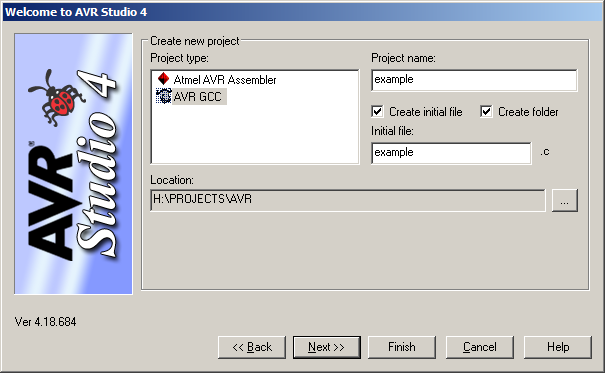
\includegraphics[scale=0.46]{newproject1}
  \caption{Eerste scherm bij aanmaken nieuw project}
  \label{fig:newproject1}
\end{figure}

\begin{figure}[h!]
  \centering
  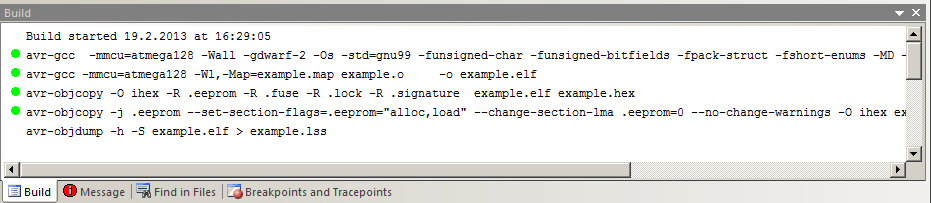
\includegraphics[scale=0.46]{atmega128gcc}
  \caption{De compiler genereert code voor de ATmega128}
  \label{fig:atmega128gcc}
\end{figure}


\section{[AS4] Vermijd gebruik van floating point.}
\label{sec:as4vermijd}
De AVR-controller heeft geen hardware voor floating point-berekeningen aan boord.
Dat betekent dat zelfs een simpele vermenigvuldiging of deling in software moet
worden ge\"{e}muleerd. En dat kost veel ruimte in Flash-ROM (programmageheugen)
en veel executietijd. Onderstaande code werd gedraaid op een ATmega16 met GNU-C
compiler versie 4.1. De floating point-berekeningen\index{ATmega16}
\index{float}
duren meer dan twee keer zo lang als de integer-berekeningen. Het gebruik van de
\index{integer}
optimalisatievlag \lstC{-O2} helpt weinig (zeg maar gewoon: niets) want de routines
voor vermenigvuldigen en delen zijn al geoptimaliseerd door de programmeurs.
Je kan veel eenvoudige floating point-delingen makkelijk omzetten naar integer-delingen
(let wel op het bereik van int's en long's) (let ook op de berekenvolgorde!):
%
\begin{equation}
\nonumber
fo = \frac{ftime}{fdiv}=\frac{ftime}{3,686} \quad \Rightarrow \quad
lo = \frac{ltime \cdot lmul}{ldiv} = \frac{ltime \cdot 1000}{3686} \qquad
\left(\frac{1}{3,686} \leftrightarrow \frac{1000}{3686}\right)
\end{equation}

\index{volatile}
\begin{lstlisting}[style=C,caption=Code met integer en floating point-berekeningen]
/* compile with -O0 and -O2 successively */

volatile float fx=13.0;
volatile float fy=23.535;
volatile float fz;

volatile long  lx=13UL;
volatile long  ly=23535;
volatile long  lz;

volatile long   ftime = 3456;
volatile float  fdiv = 3.686;
volatile float  fo;

volatile long   ltime = 3456;
volatile long   lmul = 1000;
volatile long   ldiv = 3686;
volatile long   lo;

int main() {

	fz = fy/fx;

	lz = ly/lx;

	fo = ftime/fdiv;

	lo = (ltime*lmul)/ldiv;    /* Mind parentheses!!! */

	return 0;
}
\end{lstlisting}

Let ook op het gebruik van \lstC{#define}-constanten. Constructies als

\begin{lstlisting}[style=C,numbers=none,belowcaptionskip=-12pt]
#define R_OPT (14750.0)
\end{lstlisting}

levert extreem veel code op omdat er t\'{o}ch FP-routines worden gebruikt.



%\bibliographystyle{plain}
%\bibliography{CoderenopAVR}
% Add bibliography to toc with clickable reference
\phantomsection
%\addcontentsline{toc}{section}{\bibname}
\newpage
\addcontentsline{toc}{section}{Referenties}
\printbibliography{}
 
\printindex

\end{document}
